
\chapter{Examples}
\label{chap:examples}

\section{teste}
\subsection{teste}
\subsubsection{teste}
\begin{algorithm2e}
\caption{Gauss-Seidel Algorithm}\label{alg:gauss-seidel}
\KwIn
{%
scalar $\epsilon$,
matrix $\mathbf{A} = (a_{ij})$,
vector $\vec{b}$
and initial vector $\vec{x}^{(0)}$
}
\For{$k\leftarrow 1$ \KwTo maximum iterations}
{
\For{$i\leftarrow 1$ \KwTo $n$}
{
$
x_i^{(k)} =
\frac
{
b_i-\sum_{j=1}^{i-1}a_{ij}x_j^{(k)}
-\sum_{j=i+1}^{n}a_{ij}x_j^{(k-1)}
}%
{a_{ii}}
$\;
}
\If{$\lvert\vec{x}^{(k)}-\vec{x}^{(k-1)}\rvert < \epsilon$}
{Stop}
}
\end{algorithm2e}

% \begin{table}[H]
%   \centering
%   \caption{table}
%   \begin{tabular}{cc}
%     \label{tab:tab1}
%     \hypertarget{tab:1}{}
%     Transição&Significado\\
%     \hline \\
%     \hyperlink{partialNet:t1}{\hypertarget{partialTable:t1}{$t_{1}$}}&Test\\
%     \hyperlink{partialNet:p1}{\hypertarget{partialTable:p1}{$p_{1}$}}&balbalbal\\
%     \hyperlink{partialNet:p0m2}{\hypertarget{partialTable:p0m2}{$p_{0}$}}&balbalbal
%   \end{tabular}
% \end{table}

% \newpage
% \begin{figure}[h]
%   \centering
%   \begin{tikzpicture}[>=latex',line join=bevel,]
%%
\node (p0m2) at (27.0bp,18.0bp) [draw,ellipse,place, tokens=2, label=above:, label=left:\hyperlink{partialTable:p0m2}{\hypertarget{partialNet:p0m2}{$p_{0}$}},rotate=90] {};
  \node (tt1) at (114.0bp,18.0bp) [draw,ellipse,timedtransition, label=above:, label=left:\hyperlink{partialTable:tt1}{\hypertarget{partialNet:tt1}{$t_{1}$}},rotate=90] {};
  \node (ep1) at (185.0bp,18.0bp) [draw,ellipse,extPlace, label=above:, label=left:\hyperlink{partialNet:p1}{$p_{1}$},rotate=90] {};
  \draw [-Latex,inhibitor] (p0m2) ..controls (54.05bp,18.0bp) and (76.966bp,18.0bp)  .. (tt1);
  \definecolor{strokecol}{rgb}{0.0,0.0,0.0};
  \pgfsetstrokecolor{strokecol}
  \draw (70.5bp,27.0bp) node {3};
  \draw [-Latex] (tt1) ..controls (141.25bp,18.0bp) and (147.94bp,18.0bp)  .. (ep1);
%
\end{tikzpicture}

%   \caption{example }
%   \label{fig:example}
% \end{figure}

% \newpage
% \begin{figure}[h]
%   \centering
%   \begin{tikzpicture}[>=latex',line join=bevel,]
%%
\node (et1) at (27.0bp,18.0bp) [draw,ellipse,extTransition, label=above:, label=left:\hyperlink{partialNet:t1}{$t_{1}$},rotate=90] {};
  \node (p1) at (95.0bp,18.0bp) [draw,ellipse,place, label=above:, label=left:\hyperlink{partialTable:p1}{\hypertarget{partialNet:p1}{$p_{1}$}},rotate=90] {};
  \draw [-Latex] (et1) ..controls (54.266bp,18.0bp) and (57.727bp,18.0bp)  .. (p1);
%
\end{tikzpicture}

%   \caption{example }
%   \label{fig:example}
% \end{figure}

% \newpage

% \begin{figure}[H]
%   \centering
%   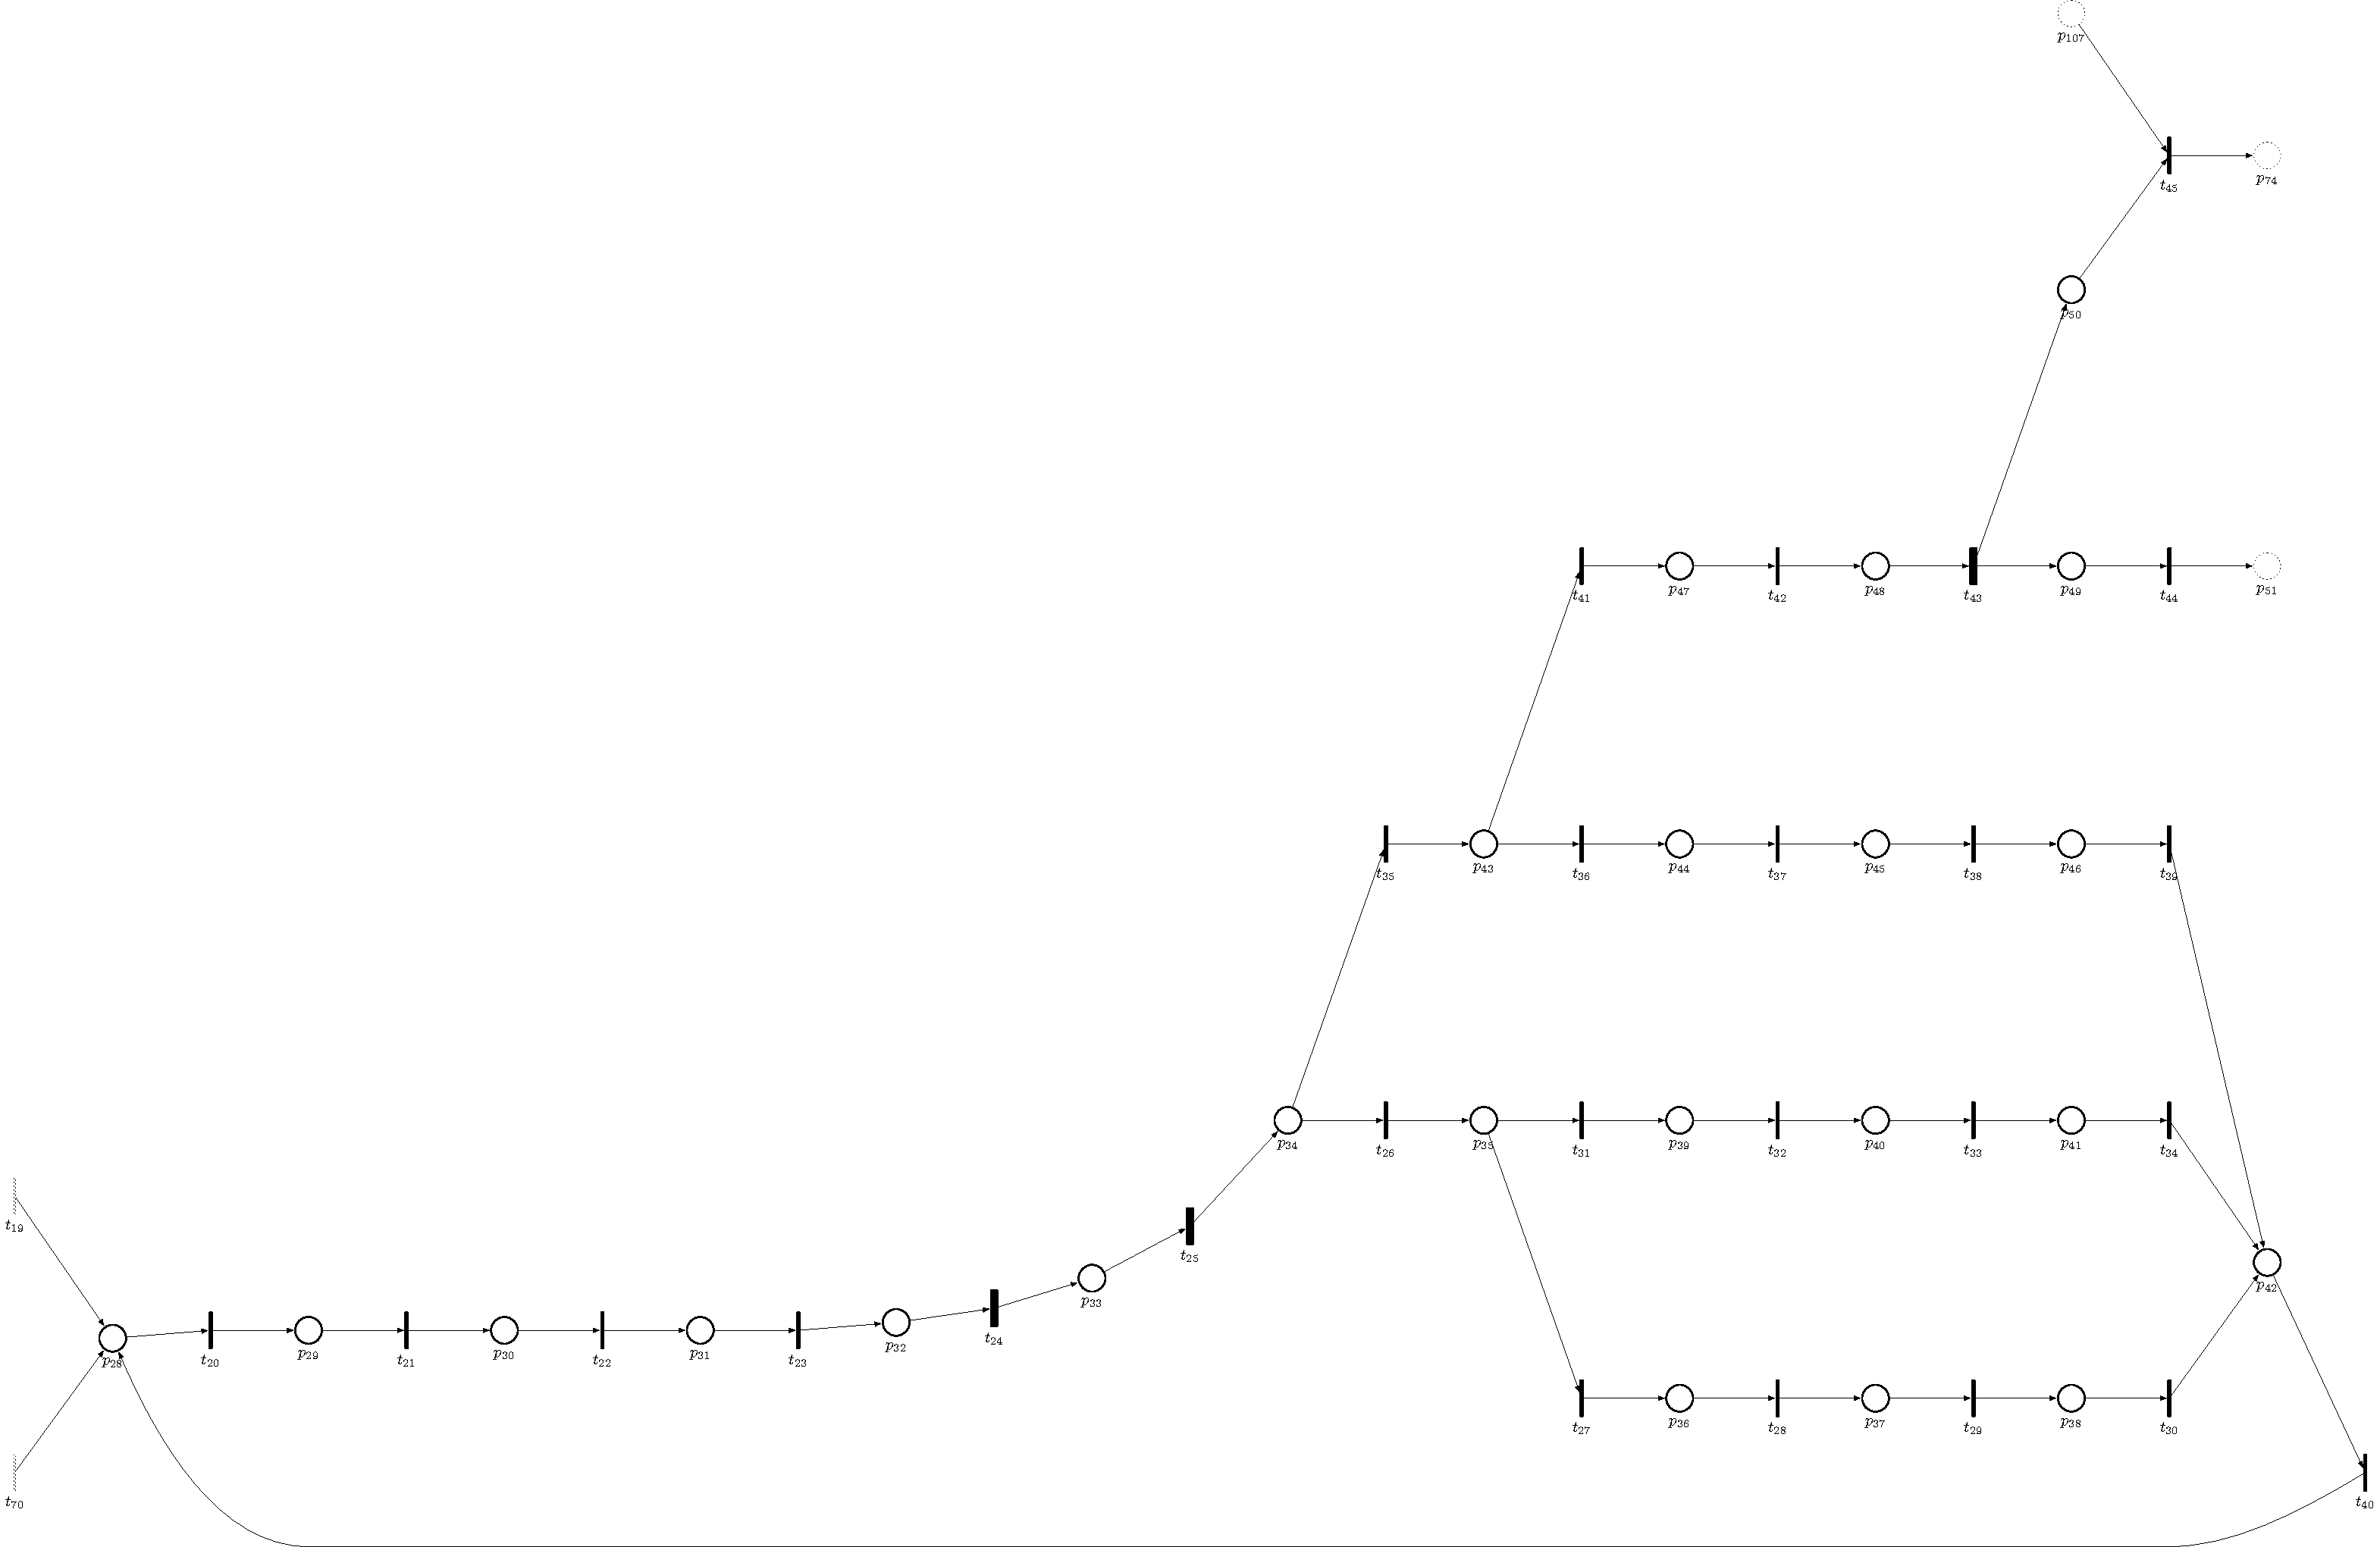
\includegraphics{../../figures/petriNets/dot/2-metalv/metalv.pdf}
%   \caption{qlksdjf}
%   \label{fig:example}
% \end{figure}


\OmegaSet

\begin{figure}[H]
  \centering
  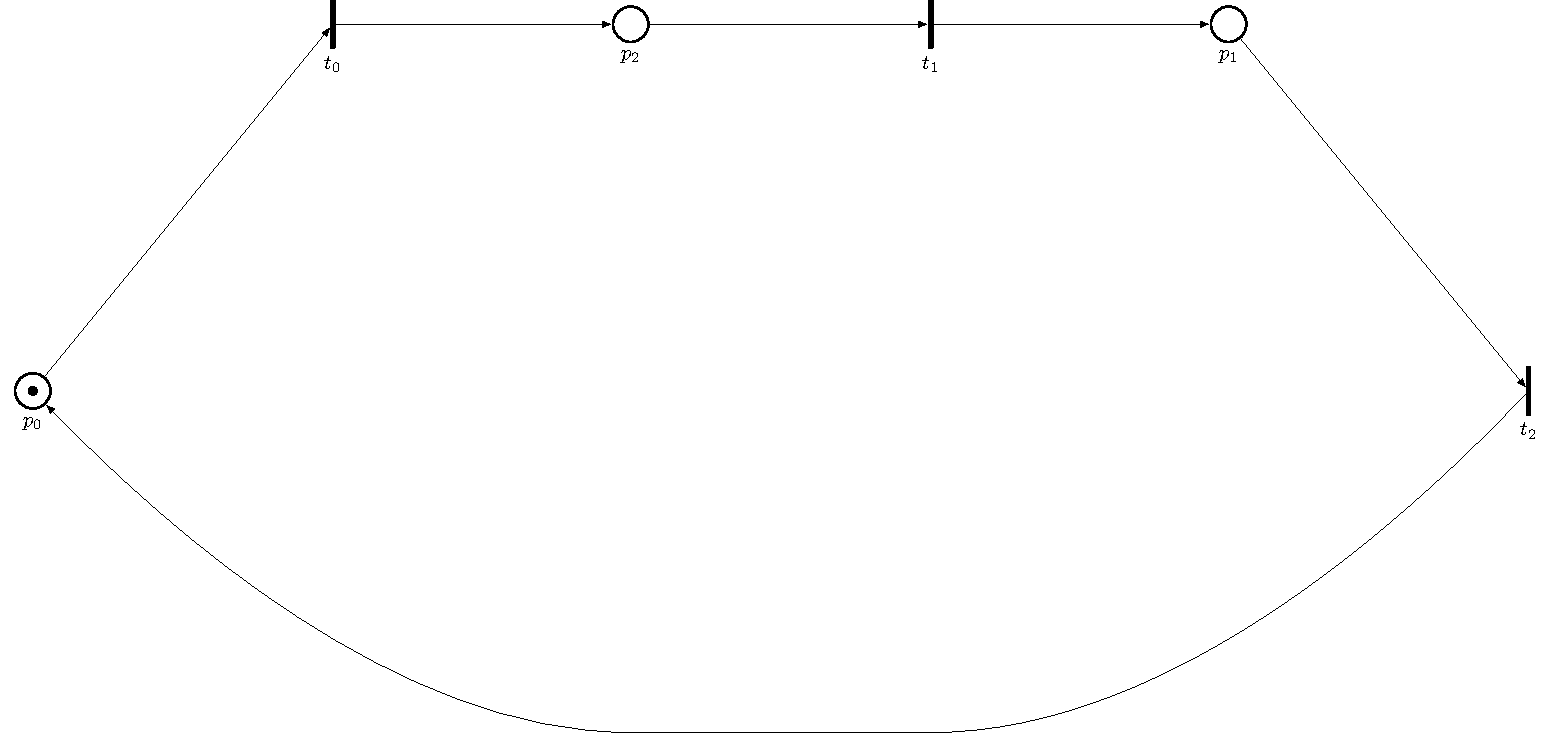
\includegraphics[width=0.4\textwidth]{../../figures/tests/teste.tikz}
  \caption{petri net example}
  \label{fig:petrinetexample}
\end{figure}


\clearpage

\addtikzfigure{../../figures/petriNets/dot/1-initialization/initial}
{Petri net of Initialization module.}
{petriinitialization}

\begin{table}[htbp]
\caption{Lugares do Módulo de Inicialização}
\centering
\begin{tabular}{c|c}
Places & Meaning\\
\hline
p\textsubscript{0} & System Stopped\\
p\textsubscript{1} & Retract MAG 1 Cylinder *\\
p\textsubscript{2} & MAG1's Cylinder Retracted\\
p\textsubscript{3} & Retract MAG 2 Cylinder *\\
p\textsubscript{4} & MAG2's Cylinder Recuado\\
p\textsubscript{5} & Retrair pistão de descarte D*\\
p\textsubscript{6} & Pistão de descarte D Recuado\\
p\textsubscript{7} & Retrair pistão de descarte C*\\
p\textsubscript{8} & Pistão de descarte C Recuado\\
p\textsubscript{9} & Retrair pistão de descarte E*\\
p\textsubscript{10} & Pistão de descarte E Recuado\\
p\textsubscript{11} & Ligar esteira sentido reverso\\
p\textsubscript{12} & Esteira limpa\\
p\textsubscript{13} & Resetar Variáveis\footnotemark\\
p\textsubscript{14} & Retrair atuador vertical da prensa\\
p\textsubscript{15} & Levantar porta da prensa\\
p\textsubscript{16} & Estender atuador horizontal da prensa\\
p\textsubscript{17} & Prensa pronta\\
p\textsubscript{18} & Braço retraído e armazenador de cubos retraído na horizontal\\
p\textsubscript{19} & Mover armazenador para direita\\
p\textsubscript{20} & Armazenador pronto na horizontal\\
p\textsubscript{21} & Mover armazenador para baixo\\
p\textsubscript{22} & Armazenador pronto na vertical\\
p\textsubscript{23} & Girar braço sentido antihorário\footnotemark\\
p\textsubscript{24} & Braço parado\\
p\textsubscript{25} & Girar braço sentido horário\textsuperscript{\ref{org074bf9c}} e Habilita HSC\\
p\textsubscript{26} & Braço parado frente a esteira\\
p\textsubscript{27} & Sistema Pronto\\
\end{tabular}
\end{table}\footnotetext[1]{\label{org10fa1d9}Variáveis IEC\textsubscript{COUNTER}, IEC\textsubscript{COUNTER1}, IEC\textsubscript{COUNTER2}, IEC\textsubscript{COUNTER3}, IEC\textsubscript{COUNTER4}, IEC\textsubscript{COUNTER5}.}\footnotetext[2]{\label{org074bf9c}Verificar sentido de rotação do braço.}

\begin{table}[htbp]
\caption{Transições do Módulo de Inicialização}
\centering
\begin{tabular}{ll}
Transitions & Meaning\\
t\textsubscript{0} & Botão de inicialização\\
t\textsubscript{1} & Sensor MAG 1 Retraído\\
t\textsubscript{2} & Sensor MAG 2 Retraído\\
t\textsubscript{3} & Sensor pistão de descarte D Retraído\\
t\textsubscript{4} & Sensor pistão de descarte C Retraído\\
t\textsubscript{5} & Sensor pistão de descarte E Retraído\\
t\textsubscript{6} & \\
t\textsubscript{7} & T=15s\\
t\textsubscript{8} & T=2.5s\\
t\textsubscript{9} & Sensor porta prensa aberta\\
t\textsubscript{10} & Sensor atuador horizontal da prensa estendido\\
t\textsubscript{11} & Sensor Hz armazenador de cubos e braço retraídos\\
t\textsubscript{12} & Fim de curso direito do armazenador de cubos\\
t\textsubscript{13} & Fim de curso inferior do armazenador de cubos\\
t\textsubscript{14} & T=2s\\
t\textsubscript{15} & Sensor Indutivo do braço\\
t\textsubscript{16} & T=1s\\
t\textsubscript{17} & Count\_300C.DB.Countval = \todo{-1690}\\
t\textsubscript{18} & \\
t\textsubscript{19} & Botão Começar\\
\end{tabular}
\end{table}


\addtikzfigure{../../figures/petriNets/dot/2-metalv/metalv}
{Petri net of metal cube half sorting module.}
{petri_initialization}

\begin{table}[htbp]
\caption{Lugares do Módulo 2 pt 1}
\centering
\begin{tabular}{ll}
p\textsubscript{28} & Mag1 vazio\\
p\textsubscript{29} & Mag1 com peça\\
p\textsubscript{30} & Estender Mag1 Horizontal*\\
p\textsubscript{31} & Retrair Mag1 Horizontal*\\
p\textsubscript{32} & Mag1 Horizontal retraído\\
p\textsubscript{33} & Ligar esteira sentido normal\\
p\textsubscript{34} & \\
p\textsubscript{35} & Peça de Plástico\\
p\textsubscript{36} & Ligar esteira sentido normal\\
p\textsubscript{37} & Estender Pistão de descarte D*\\
p\textsubscript{38} & Retrair Pistão de descarte D*\\
p\textsubscript{39} & Ligar esteira sentido normal\\
p\textsubscript{40} & Estender Pistão de descarte C*\\
p\textsubscript{41} & Retrair Pistão de descarte C*\\
p\textsubscript{42} & \\
p\textsubscript{43} & Peça de Metal\\
p\textsubscript{44} & Ligar esteira sentido normal\\
p\textsubscript{45} & Estender Pistão de descarte E*\\
p\textsubscript{46} & Retrair Pistão de descarte E*\\
p\textsubscript{47} & Ligar esteira sentido normal\\
p\textsubscript{48} & Ligar esteira sentido normal\\
p\textsubscript{49} & Peça Metal Pronta\\
p\textsubscript{50} & Esteira Parada\\
\end{tabular}
\end{table}


\begin{table}[htbp]
\caption{Transições do Módulo 2 pt 1}
\centering
\begin{tabular}{ll}
t\textsubscript{20} & \(\overline{\mbox{Sensor Chave de Presença de Peça Mag1}}\)\\
t\textsubscript{21} & \\
t\textsubscript{22} & Mag1 Horizontal estendido \(\uparrow\)\\
t\textsubscript{23} & Mag1 Horizontal retraído \(\uparrow\)\\
t\textsubscript{24} & T=0.5s\\
t\textsubscript{25} & Presença \(\uparrow\) T=0.5s\\
t\textsubscript{26} & \(\overline{\mbox{Sensor Metal}}\)\\
t\textsubscript{27} & Sensor Preto\\
t\textsubscript{28} & Presença Pistão de D \(\uparrow\)\\
t\textsubscript{29} & Sensor pistão de descarte D estendido\\
t\textsubscript{30} & Sensor pistão de descarte D retraído\\
t\textsubscript{31} & Sensor Branco\\
t\textsubscript{32} & Presença Pistão de C \(\uparrow\)\\
t\textsubscript{33} & Sensor pistão de descarte C estendido\\
t\textsubscript{34} & Sensor pistão de descarte C retraído\\
t\textsubscript{35} & Sensor Metal\\
t\textsubscript{36} & Sensor peça concavidade para baixo\\
t\textsubscript{37} & Presença Pistão de E \(\uparrow\)\\
t\textsubscript{38} & Sensor pistão de descarte E estendido\\
t\textsubscript{39} & Sensor pistão de descarte E retraído\\
t\textsubscript{40} & \\
t\textsubscript{41} & Sensor peça concavidade para cima\\
t\textsubscript{42} & Sensor final da esteira \(\uparrow\)\\
t\textsubscript{43} & T=0.5s\\
t\textsubscript{44} & Sensor final da esteira \(\downarrow\)\\
t\textsubscript{45} & \\
\end{tabular}
\end{table}


\addtikzfigure{../../figures/petriNets/dot/3-plastic^/plastic}
{Petri net of plastic cube half sorting module.}
{petri_initialization}

\begin{table}[htbp]
\caption{Lugares do Módulo 2 pt 2}
\centering
\begin{tabular}{ll}
P\textsubscript{51} & Mag2 vazio\\
P\textsubscript{52} & Mag2 com peça\\
P\textsubscript{53} & Estender Mag2 Horizontal*\\
p\textsubscript{54} & Retrair Mag2 Horizontal*\\
p\textsubscript{55} & Mag2 Horizontal Retraído\\
p\textsubscript{56} & Ligar esteira sentido normal\\
p\textsubscript{57} & \\
p\textsubscript{58} & Ligar esteira sentido normal\\
p\textsubscript{59} & Estender Pistão de descarte E*\\
p\textsubscript{60} & Retrair Pistão de descarte E*\\
p\textsubscript{61} & Peça de Metal\\
p\textsubscript{62} & Ligar esteira sentido normal\\
p\textsubscript{63} & Estender Pistão de descarte D*\\
p\textsubscript{64} & Retrair Pistão de descarte D*\\
p\textsubscript{65} & Peça Branca\\
p\textsubscript{66} & Ligar esteira sentido normal\\
p\textsubscript{67} & Estender Pistão de descarte C*\\
p\textsubscript{68} & Retrair Pistão de descarte C*\\
p\textsubscript{69} & \\
p\textsubscript{70} & Ligar esteira sentido normal\\
p\textsubscript{71} & Ligar esteira sentido normal\\
p\textsubscript{72} & Peça branca pronta\\
p\textsubscript{73} & Esteira parada\\
\end{tabular}
\end{table}

\begin{table}[htbp]
\caption{Transições do Módulo 2 pt 2}
\centering
\begin{tabular}{ll}
t\textsubscript{46} & \(\overline{\mbox{Sensor Chave de Presença de Peça Mag2}}\)\\
t\textsubscript{47} & \\
t\textsubscript{48} & Mag2 Horizontal estendido \(\uparrow\)\\
t\textsubscript{49} & Mag2 Horizontal retraído \(\uparrow\)\\
t\textsubscript{50} & T=0.5s\\
t\textsubscript{51} & Presença \(\uparrow\) T=0.5s\\
t\textsubscript{52} & Sensor Metal\\
t\textsubscript{53} & Presença Pistão de E \(\uparrow\)\\
t\textsubscript{54} & Sensor pistão de descarte E estendido\\
t\textsubscript{55} & Sensor pistão de descarte E retraído\\
t\textsubscript{56} & \(\overline{\mbox{Sensor Metal}}\)\\
t\textsubscript{57} & Sensor Preto\\
t\textsubscript{58} & Presença Pistão de D \(\uparrow\)\\
t\textsubscript{59} & Sensor pistão de descarte D estendido\\
t\textsubscript{60} & Sensor pistão de descarte D retraído\\
t\textsubscript{61} & Sensor Branco\\
t\textsubscript{62} & Sensor peça concavidade para cima\\
t\textsubscript{63} & Presença Pistão de C \(\uparrow\)\\
t\textsubscript{64} & Sensor pistão de descarte C estendido\\
t\textsubscript{65} & Sensor pistão de descarte C retraído\\
t\textsubscript{66} & \\
t\textsubscript{67} & Sensor peça concavidade para baixo\\
t\textsubscript{68} & Sensor final da esteira \(\uparrow\)\\
t\textsubscript{69} & T=0.5s\\
t\textsubscript{70} & Sensor final da esteira \(\downarrow\)\\
t\textsubscript{71} & \\
\end{tabular}
\end{table}


\addtikzfigure{../../figures/petriNets/dot/4-armBeltToPress/armBeltToPress}
{Petri net of manipulator taking a cube half from conveyor belt to assembly unit
  module.}
{petri_initialization}

\begin{table}[htbp]
\caption{Lugares do Módulo Braço Esteira Prensa}
\centering
\begin{tabular}{c|c}
Places & Meaning\\
\hline
\hyperlink{partialNet:p74}{\hypertarget{partialTable:p74}{$p_{74}$}} & Estender verticalmente o braço\\
\hyperlink{partialNet:p75}{\hypertarget{partialTable:p75}{$p_{75}$}} & Estender vertical e horizontalmente o braço e Ligar o vácuo\\
\hyperlink{partialNet:p76}{\hypertarget{partialTable:p76}{$p_{76}$}} & Estender horizontalmente o braço e Ligar o vácuo\\
\hyperlink{partialNet:p77}{\hypertarget{partialTable:p77}{$p_{77}$}} & Estender vertical e horizontalmente o braço e Ligar o vácuo\\
\hyperlink{partialNet:p78}{\hypertarget{partialTable:p78}{$p_{78}$}} & Estender verticalmente o braço e Ligar o vácuo\\
\hyperlink{partialNet:p79}{\hypertarget{partialTable:p79}{$p_{79}$}} & Habilita HSC e Estender verticalmente o braço, Ligar o vácuo e Girar Braço no sentido horário\\
\hyperlink{partialNet:p80}{\hypertarget{partialTable:p80}{$p_{80}$}} & Estender vertical e horizontalmente o braço e Ligar o vácuo\\
\hyperlink{partialNet:p81}{\hypertarget{partialTable:p81}{$p_{81}$}} & Estender horizontalmente o braço e Ligar o vácuo\\
\hyperlink{partialNet:p82}{\hypertarget{partialTable:p82}{$p_{82}$}} & Estender horizontalmente o braço\\
\hyperlink{partialNet:p83}{\hypertarget{partialTable:p83}{$p_{83}$}} & Estender vertical e horizontalmente o braço\\
\hyperlink{partialNet:p84}{\hypertarget{partialTable:p84}{$p_{84}$}} & Estender verticalmente o braço\\
\hyperlink{partialNet:p85}{\hypertarget{partialTable:p85}{$p_{85}$}} & Habilita HSC e Estender verticalmente o braço e Girar Braço no sentido antihorário\\
\hyperlink{partialNet:p86}{\hypertarget{partialTable:p86}{$p_{86}$}} & Estender Verticalmente o braço e IEC\(_{\text{COUNTER}}\):=IEC\(_{\text{COUNTER}}\)+1\\
\end{tabular}
\end{table}

\begin{table}[htbp]
\caption{Transições do Módulo Braço Esteira Prensa}
\centering
\begin{tabular}{c|c}
Transitions & Meaning\\
\hline
\hyperlink{partialNet:t72}{\hypertarget{partialTable:t72}{$t_{72}$}} & Sensor vertical braço estendido\\
\hyperlink{partialNet:tt73}{\hypertarget{partialTable:tt73}{$t_{73}$}} & T=1.5s\\
\hyperlink{partialNet:tt74}{\hypertarget{partialTable:tt74}{$t_{74}$}} & T=1.5s e Sensor vertical braço retraído\\
\hyperlink{partialNet:tt75}{\hypertarget{partialTable:tt75}{$t_{75}$}} & T=1.5s e Sensor vertical braço estendido\\
\hyperlink{partialNet:tt76}{\hypertarget{partialTable:tt76}{$t_{76}$}} & T=1.5s e Sensor vertical braço estendido\\
\hyperlink{partialNet:t77}{\hypertarget{partialTable:t77}{$t_{77}$}} & Count\_300C.DB.CountVal = \todo{-3330}\\
\hyperlink{partialNet:tt78}{\hypertarget{partialTable:tt78}{$t_{78}$}} & T=1.5s e Sensor vertical braço estendido\\
\hyperlink{partialNet:tt79}{\hypertarget{partialTable:tt79}{$t_{79}$}} & T=1.5s e Sensor vertical braço retraído\\
\hyperlink{partialNet:tt80}{\hypertarget{partialTable:tt80}{$t_{80}$}} & T=1.5s\\
\hyperlink{partialNet:tt81}{\hypertarget{partialTable:tt81}{$t_{81}$}} & T=1.5s e Sensor vertical braço estendido\\
\hyperlink{partialNet:t82}{\hypertarget{partialTable:t82}{$t_{82}$}} & IEC\(_{\text{COUNTER0.DB}}\)=1 e Sensor Hz prensa estendido e porta prensa aberta\\
\hyperlink{partialNet:tt83}{\hypertarget{partialTable:tt83}{$t_{83}$}} & T=1.5s e IEC\(_{\text{COUNTER0.DB}}\)=0 e Sensor vertical braço estendido\\
\hyperlink{partialNet:t84}{\hypertarget{partialTable:t84}{$t_{84}$}} & Count\_300C.DB.CountVal = \todo{-1690}\\
\hyperlink{partialNet:t85}{\hypertarget{partialTable:t85}{$t_{85}$}} & \\
\end{tabular}
\end{table}

 
\addtikzfigure{../../figures/petriNets/dot/5-press/press}
{Petri net of assembly unit module.}
{petri_initialization}

\begin{table}[htbp]
\caption{Lugares do Módulo prensa cubo}
\centering
\begin{tabular}{c|c}
Places & Meaning\\
\hline
\hyperlink{partialNet:p87}{\hypertarget{partialTable:p87}{$p_{87}$}} & Retrair atuador horizontal prensa*\\
\hyperlink{partialNet:p88}{\hypertarget{partialTable:p88}{$p_{88}$}} & Fechar Porta prensa*\\
\hyperlink{partialNet:p89}{\hypertarget{partialTable:p89}{$p_{89}$}} & Estender atuador vertical prensa*\\
\hyperlink{partialNet:p90}{\hypertarget{partialTable:p90}{$p_{90}$}} & Retrair atuador vertical prensa*\\
\hyperlink{partialNet:p91}{\hypertarget{partialTable:p91}{$p_{91}$}} & Abrir Porta prensa*\\
\hyperlink{partialNet:p92}{\hypertarget{partialTable:p92}{$p_{92}$}} & Estender atuador horizontal prensa*\\
\hyperlink{partialNet:p93}{\hypertarget{partialTable:p93}{$p_{93}$}} & Cubo pronto\\
\hyperlink{partialNet:p94}{\hypertarget{partialTable:p94}{$p_{94}$}} & Estender horizontalmente o braço e Ligar Vácuo\\
\hyperlink{partialNet:p95}{\hypertarget{partialTable:p95}{$p_{95}$}} & Estender verticalmente o braço\\
 & \\
\end{tabular}
\end{table}

\begin{center}
\begin{tabular}{c|c}
Transitions & Meaning\\
\hline
\hyperlink{partialNet:tt86}{\hypertarget{partialTable:tt86}{$t_{86}$}} & T=1s e Sensosr horizontal prensa retraído\\
\hyperlink{partialNet:tt87}{\hypertarget{partialTable:tt87}{$t_{87}$}} & T=1s e Sensor porta fechada\\
\hyperlink{partialNet:tt88}{\hypertarget{partialTable:tt88}{$t_{88}$}} & T=1s\\
\hyperlink{partialNet:tt89}{\hypertarget{partialTable:tt89}{$t_{89}$}} & T=1s\\
\hyperlink{partialNet:tt90}{\hypertarget{partialTable:tt90}{$t_{90}$}} & T=1s e sensor porta aberta\\
\hyperlink{partialNet:tt91}{\hypertarget{partialTable:tt91}{$t_{91}$}} & T=1s e sensor horizontal prensa estendido\\
\hyperlink{partialNet:t92}{\hypertarget{partialTable:t92}{$t_{92}$}} & \\
\hyperlink{partialNet:tt93}{\hypertarget{partialTable:tt93}{$t_{93}$}} & T=1.5s e Sensor horizontal do braço estendido\\
\end{tabular}
\end{center}


\addtikzfigure{../../figures/petriNets/dot/6-armPressToStorage/armPressToStorage}
{Petri net of manipulator taking cube from assembly unit to storage module.}
{petri_initialization}

\begin{table}[htbp]
\caption{Lugares do Módulo braço prensa armazenador}
\centering
\begin{tabular}{ll}
Places & Meaning\\
\hline
\hyperlink{partialNet:p96}{\hypertarget{partialTable:p96}{$p_{96}$}} & Estender horizontalmente o braço e Ligar Vácuo\\
\hyperlink{partialNet:p97}{\hypertarget{partialTable:p97}{$p_{97}$}} & Estender vertical e horizontalmente o braço e Ligar Vácuo\\
\hyperlink{partialNet:p98}{\hypertarget{partialTable:p98}{$p_{98}$}} & Resetar IEC\(_{\text{COUNTER0}}\)*, estender verticalmente o braço e Ligar Vácuo\\
\hyperlink{partialNet:p99}{\hypertarget{partialTable:p99}{$p_{99}$}} & Habilita HSC e Estender verticalmente o braço, Ligar Vácuo e Girar o Braço no sentido horário\\
\hyperlink{partialNet:p100}{\hypertarget{partialTable:p100}{$p_{100}$}} & Estender vertical e horizontalmente o braço e Ligar Vácuo\\
\hyperlink{partialNet:p101}{\hypertarget{partialTable:p101}{$p_{101}$}} & Estender horizontalmente o braço e Ligar Vácuo\\
\hyperlink{partialNet:p102}{\hypertarget{partialTable:p102}{$p_{102}$}} & Estender horizontalmente o braço\\
\hyperlink{partialNet:p103}{\hypertarget{partialTable:p103}{$p_{103}$}} & Estender vertical e horizontalmente o braço\\
\hyperlink{partialNet:p104}{\hypertarget{partialTable:p104}{$p_{104}$}} & Girar o braço no sentido antihorário\\
\hyperlink{partialNet:p105}{\hypertarget{partialTable:p105}{$p_{105}$}} & Braço parado\\
\hyperlink{partialNet:p106}{\hypertarget{partialTable:p106}{$p_{106}$}} & Habilita HSC e Girar o braço no sentido horário\\
\hyperlink{partialNet:p107}{\hypertarget{partialTable:p107}{$p_{107}$}} & Braço na esteira\\
\end{tabular}
\end{table}

\begin{table}[htbp]
\caption{Transições do Módulo braço prensa armazenador}
\centering
\begin{tabular}{ll}
Transitions & Meaning\\
\hline
\hyperlink{partialNet:tt94}{\hypertarget{partialTable:tt94}{$t_{94}$}} & T=1.5s e Sensor vertical braço retraído\\
\hyperlink{partialNet:t95}{\hypertarget{partialTable:t95}{$t_{95}$}} & Sensor vertical braço estendido, Fim de curso inferior e direito armazenador\\
\hyperlink{partialNet:t96}{\hypertarget{partialTable:t96}{$t_{96}$}} & \\
\hyperlink{partialNet:t97}{\hypertarget{partialTable:t97}{$t_{97}$}} & Count\_300C.DB.CountVal = \todo{-4920}\\
\hyperlink{partialNet:tt98}{\hypertarget{partialTable:tt98}{$t_{98}$}} & T=2s\\
\hyperlink{partialNet:tt99}{\hypertarget{partialTable:tt99}{$t_{99}$}} & T=2s\\
\hyperlink{partialNet:t100}{\hypertarget{partialTable:t100}{$t_{100}$}} & Sensor vertical braço retraído\\
\hyperlink{partialNet:t101}{\hypertarget{partialTable:t101}{$t_{101}$}} & Sensor vertical braço estendido, Fim de curso inferior e direito armazenador\\
\hyperlink{partialNet:t102}{\hypertarget{partialTable:t102}{$t_{102}$}} & Sensor indutivo do braço\\
\hyperlink{partialNet:tt103}{\hypertarget{partialTable:tt103}{$t_{103}$}} & T=1s\\
\hyperlink{partialNet:t104}{\hypertarget{partialTable:t104}{$t_{104}$}} & Count\_300C.DB.CountVal = \todo{-1690}\\
\end{tabular}
\end{table}


\addtikzfigure{../../figures/petriNets/dot/7-storageY/storageY}
{Petri net of storage unit positioning module (y axis).}
{petri_initialization}

\begin{table}[htbp]
\caption{Storage Unit (Y axis) Module Places.}
\centering
\begin{tabular}{cc}
Places & Meaning\\
\hline
\hyperlink{partialNet:p108}{\hypertarget{partialTable:p108}{$p_{108}$}} & Cube on Storage Unit\\
\hyperlink{partialNet:p109}{\hypertarget{partialTable:p109}{$p_{109}$}} & Move Storage Unit to the Right\\
\hyperlink{partialNet:p110}{\hypertarget{partialTable:p110}{$p_{110}$}} & \\
\hyperlink{partialNet:p111}{\hypertarget{partialTable:p111}{$p_{111}$}} & Move Storage Unit Upwards\\
\hyperlink{partialNet:p112}{\hypertarget{partialTable:p112}{$p_{112}$}} & Move Storage Unit Upwards\\
\hyperlink{partialNet:p113}{\hypertarget{partialTable:p113}{$p_{113}$}} & Move Storage Unit Upwards\\
\hyperlink{partialNet:p114}{\hypertarget{partialTable:p114}{$p_{114}$}} & Move Storage Unit Upwards\\
\hyperlink{partialNet:p115}{\hypertarget{partialTable:p115}{$p_{115}$}} & COUNTER3:=COUNTER3+1\\
\hyperlink{partialNet:p116}{\hypertarget{partialTable:p116}{$p_{116}$}} & RESET COUNTER3*\\
\hyperlink{partialNet:p117}{\hypertarget{partialTable:p117}{$p_{117}$}} & \\
\end{tabular}
\end{table}


\begin{table}[htbp]
\caption{Storage Unit (Y axis) Module Transitions.}
\centering
\begin{tabular}{cc}
Transitions & Meaning\\
\hline
\hyperlink{partialNet:tt105}{\hypertarget{partialTable:tt105}{$t_{105}$}} & T=2s\\
\hyperlink{partialNet:tt106}{\hypertarget{partialTable:tt106}{$t_{106}$}} & T=2s\\
\hyperlink{partialNet:t107}{\hypertarget{partialTable:t107}{$t_{107}$}} & COUNTER2=0\\
\hyperlink{partialNet:t108}{\hypertarget{partialTable:t108}{$t_{108}$}} & COUNTER3=4\\
\hyperlink{partialNet:t109}{\hypertarget{partialTable:t109}{$t_{109}$}} & Vertical Encoder\\
\hyperlink{partialNet:t110}{\hypertarget{partialTable:t110}{$t_{110}$}} & COUNTER2=1\\
\hyperlink{partialNet:t111}{\hypertarget{partialTable:t111}{$t_{111}$}} & COUNTER3=3\\
\hyperlink{partialNet:t112}{\hypertarget{partialTable:t112}{$t_{112}$}} & Vertical Encoder\\
\hyperlink{partialNet:t113}{\hypertarget{partialTable:t113}{$t_{113}$}} & COUNTER2=2\\
\hyperlink{partialNet:t114}{\hypertarget{partialTable:t114}{$t_{114}$}} & COUNTER3=2\\
\hyperlink{partialNet:t115}{\hypertarget{partialTable:t115}{$t_{115}$}} & Vertical Encoder\\
\hyperlink{partialNet:t116}{\hypertarget{partialTable:t116}{$t_{116}$}} & COUNTER2=3\\
\hyperlink{partialNet:t117}{\hypertarget{partialTable:t117}{$t_{117}$}} & COUNTER3=1\\
\hyperlink{partialNet:t118}{\hypertarget{partialTable:t118}{$t_{118}$}} & Vertical Encoder\\
\hyperlink{partialNet:t119}{\hypertarget{partialTable:t119}{$t_{119}$}} & \\
\hyperlink{partialNet:t120}{\hypertarget{partialTable:t120}{$t_{120}$}} & \\
\end{tabular}
\end{table}


\addtikzfigure{../../figures/petriNets/dot/8-storageX/storageX}
{Petri net of storage unit positioning module (x axis).}
{petri_initialization}

\begin{table}[htbp]
\caption{Lugares do Módulo armazenador (x)}
\centering
\begin{tabular}{ll}
p\textsubscript{120} & COUNTER1:=COUNTER1+1 e COUNTER4:=COUNTER4+1\\
p\textsubscript{121} & COUNTER5:=COUNTER5+1 e mover armazenador para a esquerda\\
p\textsubscript{122} & Reset COUNTER5*\\
p\textsubscript{123} & COUNTER5:=COUNTER5+1 e mover armazenador para a esquerda\\
p\textsubscript{124} & Reset COUNTER5*\\
p\textsubscript{125} & COUNTER5:=COUNTER5+1 e mover armazenador para a esquerda\\
p\textsubscript{126} & Reset COUNTER5*\\
p\textsubscript{127} & COUNTER5:=COUNTER5+1 e mover armazenador para a esquerda\\
p\textsubscript{128} & Reset COUNTER5*\\
p\textsubscript{129} & COUNTER5:=COUNTER5+1 e mover armazenador para a esquerda\\
p\textsubscript{130} & Reset COUNTER5*\\
p\textsubscript{131} & COUNTER5:=COUNTER5+1 e mover armazenador para a esquerda\\
p\textsubscript{132} & Reset COUNTER5*\\
p\textsubscript{133} & COUNTER5:=COUNTER5+1 e mover armazenador para a esquerda\\
p\textsubscript{134} & Reset COUNTER5* Reset COUNTER4* , COUNTER2:=COUNTER2+1\\
p\textsubscript{135} & \\
\end{tabular}
\end{table}

\begin{table}[htbp]
\caption{Transições Módulo armazenador (x)}
\centering
\begin{tabular}{ll}
t\textsubscript{119} & COUNTER4=0\\
t\textsubscript{120} & COUNTER5=1\\
t\textsubscript{121} & \\
t\textsubscript{122} & COUNTER4=1\\
t\textsubscript{123} & COUNTER5=2\\
t\textsubscript{124} & \\
t\textsubscript{125} & COUNTER4=2\\
t\textsubscript{126} & COUNTER5=3\\
t\textsubscript{127} & \\
t\textsubscript{128} & COUNTER4=3\\
t\textsubscript{129} & COUNTER5=4\\
t\textsubscript{130} & \\
t\textsubscript{131} & COUNTER4=4\\
t\textsubscript{132} & COUNTER5=5\\
t\textsubscript{133} & \\
t\textsubscript{134} & COUNTER4=5\\
t\textsubscript{135} & COUNTER5=8\\
t\textsubscript{136} & \\
t\textsubscript{137} & COUNTER4=6\\
t\textsubscript{138} & COUNTER5=9\\
t\textsubscript{139} & \\
\end{tabular}
\end{table}


\addtikzfigure{../../figures/petriNets/dot/9-storePiece/storePiece}
{Petri net of cube storage module.}
{petri_initialization}

\begin{table}[htbp]
\caption{Places from the cube storage module.}
\centering
\begin{tabular}{ll}
p\(_{\text{136}}\) & Estender horizontalmente armazenador\\
p\(_{\text{137}}\) & Estender horizontalmente armazenador e mover armazenador para baixo\\
p\(_{\text{138}}\) & Estender horizontalmente armazenador\\
p\(_{\text{139}}\) & Peça armazenada\\
p\(_{\text{140}}\) & Mover armazenador para a direita\\
p\(_{\text{141}}\) & Armazenador pronto na horizontal\\
p\(_{\text{142}}\) & Mover armazenador para baixo\\
p\(_{\text{143}}\) & Armazenador pronto na vertical\\
p\(_{\text{144}}\) & \\
p\(_{\text{145}}\) & Armazenador pronto\\
\end{tabular}
\end{table}

\begin{table}[htbp]
\caption{Transitions from the cube storage module.}
\centering
\begin{tabular}{ll}
t\(_{\text{140}}\) & T=2s\\
t\(_{\text{141}}\) & T=3s\\
t\(_{\text{142}}\) & T=0.25s\\
t\(_{\text{143}}\) & T=3s\\
t\(_{\text{144}}\) & T=7s\\
t\(_{\text{145}}\) & Fim de curso direito do armazenador\\
t\(_{\text{146}}\) & Fim de curso inferior do armazenador\\
t\(_{\text{147}}\) & \\
t\(_{\text{148}}\) & COUNTER1<28\\
t\(_{\text{149}}\) & COUNTER1=28\\
\end{tabular}
\end{table}







%%% Local Variables:
%%% mode: latex
%%% TeX-master: "../monografia"
%%% End:
